% !TeX root = ../main.tex

\section{Introduzione}
% cos'è devops, la filosofia devops, no silos, ecc
A causa della continua evoluzione delle tecnologie e all'aumento della concorrenza le aziende hanno bisogno di realizzare prodotti sempre più velocemente mantenendo e possibilmente aumentando la qualità~\cite{krief2019learning}. In risposta a questo problema è nata una vera e propria cultura, chiamata DevOps, la quale definisce sia un modo di pensare che una metodologia di lavoro fortemente basata sulla collaborazione tra i diversi team.

Fornisce infatti un insieme di pratiche al fine di ridurre le barriere tra il team di sviluppo (Dev) e il team operativo (Ops). Da un lato gli sviluppatori vogliono innovare e rilasciare software velocemente, mentre dall'altro lato l'obiettivo è quello di garantire la stabilità e la qualità dei sistemi. Oltre alla collaborazione tra i diversi team esistono altri principi alla base della cultura DevOps:
\begin{itemize}
    \item \textbf{Automazione} - L'intervento umano deve essere ridotto il più possibile al fine di ridurre gli errori e le tempistiche. In questo modo vengono rimossi tutti i compiti ripetitivi che sarebbero stati a carico dello sviluppatore facendogli risparmiare tempo.
    \item \textbf{Monitoraggio} - Deve essere possibile analizzare in ogni momento lo stato dei processi che compongono il sistema con lo scopo di reagire, prevenire e prevedere le situazioni critiche ma anche fornire feedback allo sviluppatore per aumentare la qualità del prodotto.
\end{itemize}

\section{Tecniche di automazione e vantaggi}
Ogni azienda ha i propri vincoli, requisiti e metodi i quali la rendono unica e per questo motivo non esiste un unico modo di utilizzo del DevOps. Esistono invece diverse tecniche che rispettano i principi DevOps e che possono essere applicate e adattate ad ogni azienda al fine di aumentare la qualità del software prodotto e diminuire il time-to-market (TTM)~\cite{devis2016effective}.

I principali benefici nell'adozione della cultura DevOps sono~\cite{krief2019learning}:
\begin{itemize}
    \item Migliore comunicazione e collaborazione all'interno dei team con un impatto umano e sociale a livello aziendale.
    \item Tempi di consegna in produzione minori che comportano un aumento delle performance e della soddisfazione dell'utente finale.
    \item Risparmio di tempo e risorse dovuti dall'utilizzo di un ciclo di sviluppo iterativo e tecniche di automazione.
\end{itemize}

I team che intendono adottare le tecniche DevOps nel proprio processo di sviluppo devono seguire metodologie Agile con fasi iterative che permettono maggiore qualità delle funzionalità e feedback rapidi da parte dell'utente. Le principali pratiche che vengono adottate sono: (\textit{i}) Continuous Integration, (\textit{ii}) Continuous Delivery, (\textit{iii}) Continuous Monitoring.

\begin{figure}[H]
    \centering
    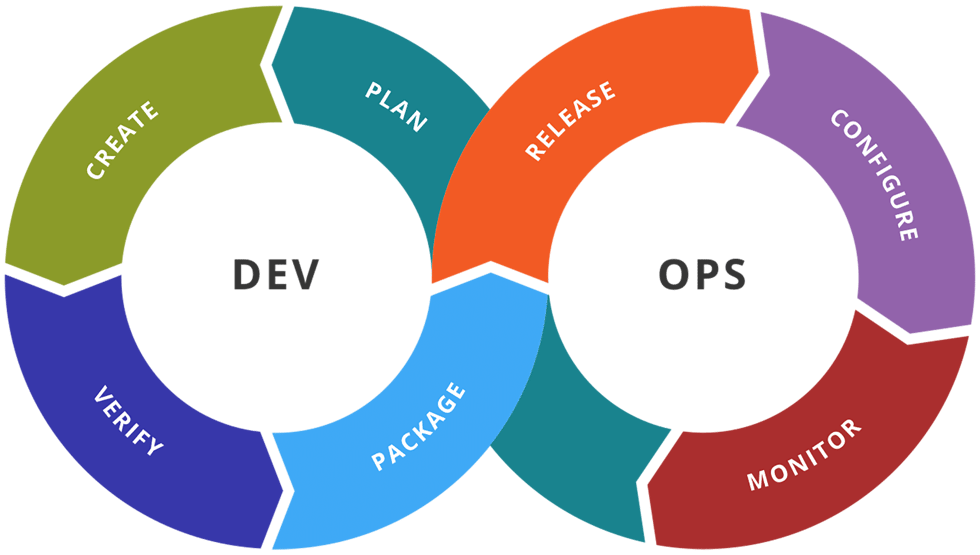
\includegraphics[width=0.6\textwidth]{img/Devops-toolchain.png}
    \caption{Fasi del ciclo di sviluppo software con tecniche DevOps.}
\end{figure}

\subsection{Continuous Integration}
Maggiore è la complessità di un progetto e maggiore è la necessità di integrare frequentemente e preventivamente i componenti software al fine di verificare che essi funzionino correttamente~\cite{duvall2007continuous}. Con Continuous Integration (CI) si intende una pratica di sviluppo software dove i membri di un team integrano frequentemente il loro lavoro e ogni integrazione è testata e verificata da un sistema automatico in grado di intercettare gli errori il più velocemente possibile\footnote{\href{https://martinfowler.com/articles/continuousIntegration.html}{https://martinfowler.com/articles/continuousIntegration.html}}.

\subsection{Continuous Delivery}

\subsection{Continuous Monitoring}

\subsection{Continuous Inspection}
% solitamente si chiama devsecops quando contiene anche automazione sull analisi automatica del codice

\section{Strumenti}
% descrizione strumenti per l'automazione in generale (gitlab runner + Pipeline as Code)
\subsection{Pipeline as Code}

\subsection{Runners}

\subsection{Software as a Service}
% descrizione strumenti as a service per l'automazione del processo (runner managed, sonarcloud, ...) e dello dello sviluppo mobile (xcode cloud, bitrise, google play console, testflight)
